\chapter{Desarrollo Teórico y Diseño del Circuito}
\label{sec:desarrollo_diseno}

\section{Amplificador de Instrumentación}

La arquitectura conceptual del amplificador de instrumentación de tres amplificadores operacionales (Figura~\ref{crkt:amp_inst_teorico}) se compone de dos etapas funcionales bien definidas: en primer lugar, una etapa de entrada diferencial con alta impedancia implementada mediante dos amplificadores operacionales ($U_1$ y $U_2$); en segundo lugar, una etapa restadora de precisión encargada de eliminar las señales de modo común, constituida por un tercer operacional ($U_3$).

\begin{figure}[!ht]
  \centering
    \begin{tikzpicture}[american, transform shape]

  % -------------------------------------------------------------
  % Entradas de señal (horizontales alineadas con los terminales +)
  % -------------------------------------------------------------
  % U1 con yscale=-1 tiene su terminal U1.+ en y = 2.99
  % U2 con yscale=1 tiene su terminal U2.+ en y = -2.99
  \node[ocirc] (in1) at (0.3, 2.99) {};
  \node[anchor=east] at (in1.west) {$e_1$};
  \node[ocirc] (in2) at (0.3, -2.99) {};
  \node[anchor=east] at (in2.west) {$e_2$};

  % -------------------------------------------------------------
  % Etapa 1: Buffers de entrada (U1 y U2)
  % -------------------------------------------------------------
  \node[op amp, yscale=-1] (U1) at (3.0, 2.5) {};
  \node at (2.8, 2.5) {$U_1$};
  \draw (in1) -- (U1.+);

  \node[op amp] (U2) at (3.0, -2.5) {};
  \node at (2.8, -2.5) {$U_2$};
  \draw (in2) -- (U2.+);

  % Nodos de terminales inversores
  \draw (U1.-) -- (1.8, 2.01);
  \draw (U2.-) -- (1.8, -2.01);

  % Impedancia Z1 entre terminales inversores
  \draw (1.8, 0.9) to[generic, l={$Z_1$}] (1.8, -0.9);
  \draw (1.8, 2.01) -- (1.8, 0.9);
  \draw (1.8, -2.01) -- (1.8, -0.9);

  % Impedancias de realimentacion Z2
  \draw (1.8, 1.3) node[circ]{} -- (2.3, 1.3)
        to[generic, l_={$Z_2$}] (3.7, 1.3)
        -- (4.2, 1.3) -- (4.2, 2.5) -- (U1.out);

  \draw (1.8, -1.3) node[circ]{} -- (2.3, -1.3)
        to[generic, l={$Z_2$}] (3.7, -1.3)
        -- (4.2, -1.3) -- (4.2, -2.5) -- (U2.out);

  % Tensiones intermedias eo1 y eo2
  \draw (U1.out) -- (4.8, 2.5) node[circ]{};
  \node[above] at (4.8, 2.5) {$e_{o1}$};
  \draw (U2.out) -- (4.8, -2.5) node[circ]{};
  \node[below] at (4.8, -2.5) {$e_{o2}$};

  % -------------------------------------------------------------
  % Etapa 2: Restador (U3)
  % -------------------------------------------------------------
  \node[op amp] (U3) at (9.0, 0.0) {};
  \node at (8.8, 0.0) {$U_3$};

  % Rama superior: eo1 -> Z3 -> entrada inversora U3.-
  \draw (4.8, 2.5) -- (5.0, 2.5)
        to[generic, l={$Z_3$}] (6.3, 2.5)
        -- (6.6, 2.5) |- (U3.-);

  % Rama inferior: eo2 -> Z3 -> entrada no inversora U3.+
  \draw (4.8, -2.5) -- (5.0, -2.5)
        to[generic, l_={$Z_3$}] (6.3, -2.5)
        -- (6.6, -2.5) |- (U3.+);

  % Realimentacion Z4 en lazo inversor (desde nodo antes de U3.- hacia U3.out)
  \draw (7.3, 0.49) node[circ]{} -- (7.3, 1.8)
        to[generic, l={$Z_4$}] (9.6, 1.8)
        -| (U3.out);
  \draw (9.6, 0.0) node[circ]{};

  % Impedancia Z4 a masa en lazo no inversor (desde nodo antes de U3.+ hacia masa)
  \draw (7.3, -0.49) node[circ]{}
        to[generic, l={$Z_4$}] (7.3, -1.9)
        node[ground]{};

  % Salida final eo
  \draw (U3.out) -- (10.6, 0.0);
  \node[ocirc] (eo) at (10.6, 0.0) {};
  \node[anchor=west] at (eo.east) {$e_o$};

\end{tikzpicture}
%
  \caption{Diagrama del circuito amplificador de instrumentación.}
  \label{crkt:amp_inst_teorico}
\end{figure}

El análisis del circuito se puede realizar a partir del estudio de cada etapa,
asumiendo amplificadores operacionales ideales en régimen lineal con
cortocircuito virtual ($v_- = v_+$) e impedancias de entrada infinitas.

En primer lugar, se analiza la segunda etapa correspondiente al restador diferencial de precisión ($U_3$) con sus impedancias balanceadas $Z_3$ y $Z_4$. Dado que la corriente de entrada al pin no inversor del operacional es nula, el potencial $v_{+3}$ queda determinado por el divisor de tensión pasivo conectado a la salida intermedia $e_{o2}$:
\begin{equation}
  v_{+3} = e_{o2} \cdot \frac{Z_4}{Z_3 + Z_4}
  \label{eq:paso1_vplus}
\end{equation}

Por otro lado, planteando la ley de corrientes de Kirchhoff en el nodo inversor $v_{-3}$ y considerando que tampoco entra corriente al pin inversor del amplificador:
\begin{equation*}
  \frac{e_{o1} - v_{-3}}{Z_3} + \frac{e_o - v_{-3}}{Z_4} = 0
\end{equation*}
Separando los términos para despejar la tensión de salida $e_o$:

\begin{equation*}
  \frac{e_o}{Z_4} = \frac{v_{-3}}{Z_4} + \frac{v_{-3}}{Z_3} - \frac{e_{o1}}{Z_3} = v_{-3} \left(\frac{1}{Z_4} + \frac{1}{Z_3}\right) - \frac{e_{o1}}{Z_3}
\end{equation*}
Multiplicando toda la igualdad por $Z_4$:
\begin{equation*}
  e_o = v_{-3} \left(1 + \frac{Z_4}{Z_3}\right) - e_{o1} \frac{Z_4}{Z_3}
\end{equation*}

\begin{equation*}
  e_o = v_{-3} \cdot \frac{Z_3 + Z_4}{Z_3} - e_{o1} \cdot \frac{Z_4}{Z_3}
\end{equation*}

Considerando la condición de cortocircuito virtual ($v_{-3} = v_{+3}$) y sustituyendo la tensión $v_{+3}$ obtenida previamente~\eqref{eq:paso1_vplus}:
\begin{equation*}
  e_o = \left(e_{o2} \cdot \frac{Z_4}{Z_3 + Z_4}\right) \cdot \left(\frac{Z_3 + Z_4}{Z_3}\right) - e_{o1} \cdot \frac{Z_4}{Z_3}
\end{equation*}
\begin{equation*}
  e_o = e_{o2} \cdot \frac{Z_4}{Z_3} - e_{o1} \cdot \frac{Z_4}{Z_3}
\end{equation*}
\begin{equation}
  e_o = (e_{o2} - e_{o1}) \cdot \frac{Z_4}{Z_3}
  \label{eq:eo_restador}
\end{equation}

Por su parte, en la primera etapa, las señales de entrada $e_1$ y $e_2$ ingresan
directamente a los terminales no inversores de los operacionales $U_1$ y $U_2$.
Por cortocircuito virtual ($v_{-1} = e_1$ y $v_{-2} = e_2$), sobre la impedancia
central $Z_1$ cae la diferencia $(e_1 - e_2)$, circulando una
corriente $i = (e_1 - e_2)/Z_1$ que fluye íntegramente a través de las ramas de
realimentación $Z_2$.

Para la componente diferencial, por simetría el punto medio de $Z_1$ se encuentra a potencial nulo (masa virtual de señal). Cada mitad del circuito queda así desacoplada con una impedancia equivalente $Z_1/2$ a masa, operando como una etapa no inversora con ganancia $1 + \frac{Z_2}{Z_1/2} = 1 + 2\frac{Z_2}{Z_1}$. Se obtienen así las expresiones desacopladas de las salidas intermedias:
\begin{equation*}
  e_{o2} = e_2 \cdot \left(1 + 2 \frac{Z_2}{Z_1}\right), \qquad e_{o1} = e_1 \cdot \left(1 + 2 \frac{Z_2}{Z_1}\right)
\end{equation*}
Restando miembro a miembro ambas salidas intermedias:
\begin{equation}
  e_{o2} - e_{o1} = (e_2 - e_1) \cdot \left(1 + 2 \frac{Z_2}{Z_1}\right)
  \label{eq:diff_salidas_etapa1}
\end{equation}

Luego, reemplazando la diferencia entre las salidas intermedias~\eqref{eq:diff_salidas_etapa1} en la ecuación del restador~\eqref{eq:eo_restador}, se obtiene la tensión de salida total del sistema:
\begin{equation*}
  e_o = (e_2 - e_1) \cdot \left(1 + 2 \frac{Z_2}{Z_1}\right) \cdot \frac{Z_4}{Z_3}
\end{equation*}
Dividiendo ambos miembros por la diferencia $(e_2 - e_1)$, se obtiene la ganancia diferencial de tensión del amplificador de instrumentación:
\begin{equation*}
  \frac{e_o}{e_2 - e_1} = \left(1 + 2 \frac{Z_2}{Z_1}\right) \cdot \frac{Z_4}{Z_3}
\end{equation*}

\section{Filtrado Pasabanda Activo}

El filtrado pasa banda suele implementarse como una etapa pasiva o activa independiente
a la salida del restador. No obstante, también se puede integrar la respuesta frecuencial
directamente en las redes de realimentación y entrada de la etapa restadora ($U_3$), según se ilustra en el circuito de
la Figura~\ref{crkt:sustitucion_z}.

\begin{figure}[!ht]
  \centering
  \resizebox{0.75\textwidth}{!}{%
    \begin{tikzpicture}[american, transform shape]

  % -------------------------------------------------------------
  % Entradas de señal (horizontales alineadas con los terminales +)
  % -------------------------------------------------------------
  % U1 con yscale=-1 tiene U1.+ en y = 3.29 (2.8 + 0.49)
  % U2 con yscale=1 tiene U2.+ en y = -3.29 (-2.8 - 0.49)
  \node[ocirc] (in1) at (0.5, 3.29) {};
  \node[anchor=east] at (in1.west) {$e_1$};
  \node[ocirc] (in2) at (0.5, -3.29) {};
  \node[anchor=east] at (in2.west) {$e_2$};

  % -------------------------------------------------------------
  % Etapa 1: Buffers con sustitucion Z1 -> R1, Z2 -> R2
  % -------------------------------------------------------------
  \node[op amp, yscale=-1] (U1) at (3.5, 2.8) {};
  \node at (3.3, 2.8) {$U_1$};
  \draw (in1) -- (U1.+);

  \node[op amp] (U2) at (3.5, -2.8) {};
  \node at (3.3, -2.8) {$U_2$};
  \draw (in2) -- (U2.+);

  % Terminales inversores
  \draw (U1.-) -- (2.3, 2.31);
  \draw (U2.-) -- (2.3, -2.31);

  % Sustitucion Z1 = R1
  \draw (2.3, 0.9) to[american resistor, l={$R_1$}] (2.3, -0.9);
  \draw (2.3, 2.31) -- (2.3, 0.9);
  \draw (2.3, -2.31) -- (2.3, -0.9);

  % Sustitucion Z2 = R2
  \draw (2.3, 1.5) node[circ]{} -- (2.8, 1.5)
        to[american resistor, l_={$R_2$}] (4.2, 1.5)
        -- (4.7, 1.5) -- (4.7, 2.8) -- (U1.out);

  \draw (2.3, -1.5) node[circ]{} -- (2.8, -1.5)
        to[american resistor, l={$R_2$}] (4.2, -1.5)
        -- (4.7, -1.5) -- (4.7, -2.8) -- (U2.out);

  % -------------------------------------------------------------
  % Etapa 2: Sustitucion Z3 -> C3 serie R3, Z4 -> R4 paralelo C4
  % -------------------------------------------------------------
  \node[op amp] (U3) at (11.0, 0.0) {};
  \node at (10.8, 0.0) {$U_3$};

  % Rama superior: Z3(s) = C3 serie R3 hacia entrada inversora U3.-
  \draw (U1.out) -- (5.2, 2.8) node[circ]{}
        to[C, l={$C_3$}] (6.6, 2.8)
        to[american resistor, l={$R_3$}] (8.3, 2.8)
        -- (8.8, 2.8) |- (U3.-);

  % Rama inferior: Z3(s) = C3 serie R3 hacia entrada no inversora U3.+
  \draw (U2.out) -- (5.2, -2.8) node[circ]{}
        to[C, l_={$C_3$}] (6.6, -2.8)
        to[american resistor, l_={$R_3$}] (8.3, -2.8)
        -- (8.8, -2.8) |- (U3.+);

  % Realimentacion Z4(s) = R4 paralelo C4 en lazo inversor
  \draw (9.5, 0.49) node[circ]{} -- (9.5, 2.3);
  \draw (9.5, 2.3) -- (9.8, 2.3) -- (9.8, 3.0)
        to[american resistor, l={$R_4$}] (11.8, 3.0)
        -- (11.8, 2.3);
  \draw (9.8, 2.3) -- (9.8, 1.6)
        to[C, l={$C_4$}] (11.8, 1.6)
        -- (11.8, 2.3);
  \draw (11.8, 2.3) -- (12.3, 2.3) -| (U3.out);
  \draw (12.3, 0.0) node[circ]{};

  % Red a masa no inversora Z4(s) = R4 paralelo C4
  \draw (9.5, -0.49) node[circ]{} -- (9.5, -1.3) -- (10.0, -1.3);
  \draw (10.0, -1.3) to[american resistor, l_={$R_4$}] (10.0, -2.6);
  \draw (10.0, -1.3) -- (11.4, -1.3)
        to[C, l={$C_4$}] (11.4, -2.6);
  \draw (10.0, -2.6) -- (11.4, -2.6);
  \draw (10.7, -2.6) node[circ]{} -- (10.7, -2.9) node[ground]{};

  % Salida filtrada e_o3
  \draw (U3.out) -- (13.0, 0.0);
  \node[ocirc] (eo3) at (13.0, 0.0) {};
  \node[anchor=west] at (eo3.east) {$e_{o3}$};

\end{tikzpicture}
%
    }
  \caption{Topología del amplificador de instrumentación con las impedancias actualizadas para filtrado pasabanda activo.}
  \label{crkt:sustitucion_z}
\end{figure}

Para ello se efectúan las siguientes sustituciones de componentes en el dominio de Laplace:
\begin{itemize}
  \item $Z_1 = R_1$: Resistencia que calibra la ganancia diferencial de entrada.
  \item $Z_2 = R_2$: Resistencias de simetría en los lazos de realimentación de $U_1$ y $U_2$.
  \item $Z_3(s)$: Rama de entrada al restador, compuesta por la conexión serie de un capacitor $C_3$ y un resistor $R_3$:
  \begin{equation}
    Z_3(s) = R_3 + \frac{1}{s C_3} = \frac{s R_3 C_3 + 1}{s C_3}
    \label{eq:z3_s}
  \end{equation}
  \item $Z_4(s)$: Rama de realimentación e impedancia a masa, formada por la conexión en paralelo de un resistor $R_4$ y
  un capacitor $C_4$:
  \begin{equation}
    Z_4(s) = R_4 \parallel \frac{1}{s C_4} = \frac{R_4}{s R_4 C_4 + 1}
    \label{eq:z4_s}
  \end{equation}
\end{itemize}

Para preservar el balance del restador y garantizar la máxima atenuación de modo común, las dos ramas de entrada al
operacional $U_3$ deben ser rigurosamente idénticas ($Z_3 = Z'_3$ y $Z_4 = Z'_4$). Bajo esta condición de puente balanceado
y aplicando en el dominio transformado de Laplace la relación del restador deducida en~\eqref{eq:eo_restador}, la salida de
la etapa $U_3$ viene dada por:
\begin{equation}
  e_{o3}(s) = (e_{o2}(s) - e_{o1}(s)) \frac{Z_4(s)}{Z_3(s)}
  \label{eq:salida_u3}
\end{equation}

Dividiendo las ecuaciones de impedancia~\eqref{eq:z4_s} y~\eqref{eq:z3_s}:
\begin{equation*}
  \frac{Z_4(s)}{Z_3(s)} = \frac{\dfrac{R_4}{s R_4 C_4 + 1}}{\dfrac{s R_3 C_3 + 1}{s C_3}} = \frac{s R_4 C_3}{(s R_3 C_3 + 1)(s R_4 C_4 + 1)}
\end{equation*}

Sustituyendo la diferencia de la primera etapa~\eqref{eq:diff_salidas_etapa1} en~\eqref{eq:salida_u3}, se arriba a la
función de transferencia analítica completa de las etapas 1 y 2:
\begin{equation}
  F(s) = \frac{e_{o3}(s)}{e_2(s) - e_1(s)} = \left(1 + 2 \frac{R_2}{R_1}\right) \frac{s R_4 C_3}{(s R_3 C_3 + 1)(s R_4 C_4 + 1)}
  \label{eq:ft_completa}
\end{equation}

\section{Análisis en Frecuencia y Diagrama de Bode}

La función de transferencia $F(s)$ formulada en la ecuación~\eqref{eq:ft_completa} revela de forma directa las singularidades
que moldean la respuesta en frecuencia:
\begin{enumerate}
  \item Cero en el origen ($s = 0$): Proporcionado por el término $s R_4 C_3$ en el numerador, introduce una asíntota de
  crecimiento de $+20\ \text{dB/década}$ desde frecuencias nulas. Esto asegura que la ganancia a corriente continua sea
  nula ($F(0) = 0$), eliminando por completo cualquier tensión de offset de entrada o potencial de contacto electrodo-piel.
  \item Polo inferior ($p_3$): Determinado por la constante de tiempo de la red serie de entrada:
  \begin{equation*}
    p_3 = \frac{1}{R_3 C_3} \implies f_L \approx \frac{p_3}{2 \pi} = \frac{1}{2 \pi R_3 C_3}
  \end{equation*}
  A partir de $f_L$, la respuesta cambia de $+20\ \text{dB/década}$ a pendiente horizontal ($0\ \text{dB/década}$),
  dando inicio a la banda pasante.
  \item Polo superior ($p_4$): Establecido por la constante de tiempo de la red en paralelo de realimentación:
  \begin{equation*}
    p_4 = \frac{1}{R_4 C_4} \implies f_H \approx \frac{p_4}{2 \pi} = \frac{1}{2 \pi R_4 C_4}
  \end{equation*}
  A partir de $f_H$, la respuesta cae con una pendiente asintótica de $-20\ \text{dB/década}$, atenuando interferencias de
  alta frecuencia.
\end{enumerate}

En la Figura~\ref{plot:bode_teorico} se ilustra el comportamiento frecuencial resultante, integrando el trazado asintótico ideal con la curva de respuesta real suavizada para la banda de paso delimitada entre $f_L$ y $f_H$.

\begin{figure}[!ht]
  \centering
  \resizebox{0.82\textwidth}{!}{%
    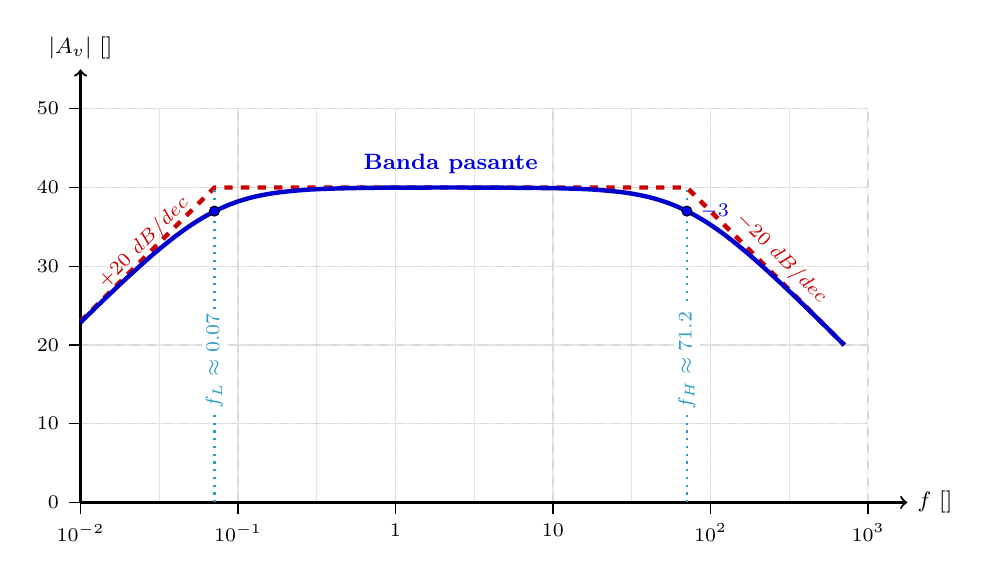
\begin{tikzpicture}[scale=1.0, transform shape]

  % Grid semilogaritmico tenue
  \draw[step=1.0, color=gray!20, thin] (0, 0) grid (10, 5);

  % Lineas de la grilla (SOLO para y > 0 y x > 0 para no superponer lineas punteadas sobre los ejes)
  \foreach \y in {1, 2, 3, 4, 5} {
    \draw[dashed, color=gray!30] (0, \y) -- (10, \y);
  }
  \foreach \x in {2, 4, 6, 8, 10} {
    \draw[dashed, color=gray!30] (\x, 0) -- (\x, 5);
  }

  % Marcas eje Y (Ganancia en dB)
  \foreach \y/\val in {0/0, 1/10, 2/20, 3/30, 4/40, 5/50} {
    \draw (0, \y) -- (-0.15, \y) node[left, font=\scriptsize] {$\val$};
  }

  % Marcas eje X (Decadas logaritmicas)
  \foreach \x/\label in {0/{$10^{-2}$}, 2/{$10^{-1}$}, 4/{$1$}, 6/{$10$}, 8/{$10^2$}, 10/{$10^3$}} {
    \draw (\x, 0) -- (\x, -0.15) node[below, font=\scriptsize] {\label};
  }

  % Ejes coordenados (dibujados solidos por encima de la grilla)
  \draw[->, thick] (0, 0) -- (10.5, 0) node[right, font=\footnotesize] {$f\ [\unit{\hertz}]$};
  \draw[->, thick] (0, 0) -- (0, 5.5) node[above, font=\footnotesize] {$|A_v|\ [\unit{\decibel}]$};

  % Curva Asintotica (linea discontinua roja)
  % fL = 0.071 Hz -> x_L = 2*(log10(0.071) + 2) = 1.70
  % fH = 71.18 Hz -> x_H = 2*(log10(71.18) + 2) = 7.70
  % Pendiente +20 dB/dec -> +1 por cada unidad de x
  \draw[dashed, ultra thick, red!80!black] 
    (0, 2.3) -- (1.70, 4.0) -- (7.70, 4.0) -- (9.70, 2.0);

  % Curva Real Suavizada (linea solida azul calculada analiticamente)
  \draw[ultra thick, blue!80!black] plot[smooth] coordinates {
    (0.00, 2.287) (0.30, 2.579) (0.60, 2.862) (0.90, 3.132) (1.20, 3.377) 
    (1.45, 3.553) (1.70, 3.697) (1.95, 3.805) (2.20, 3.880) (2.50, 3.935) 
    (2.90, 3.973) (3.40, 3.991) (4.00, 3.998) (5.00, 3.999) (6.00, 3.991) 
    (6.50, 3.974) (6.90, 3.937) (7.20, 3.882) (7.45, 3.808) (7.70, 3.701) 
    (7.95, 3.559) (8.20, 3.384) (8.50, 3.140) (8.80, 2.871) (9.10, 2.588) 
    (9.40, 2.296) (9.70, 2.000)
  };

  % Lineas de corte y singularidades con etiquetas verticales sobre las lineas
  \draw[dotted, thick, color=cyan!80!black] (1.70, 0) -- (1.70, 4.0);
  \node[fill=white, inner sep=1.5pt, font=\scriptsize, text=cyan!80!black, rotate=90] at (1.70, 1.8) {$f_L \approx \SI{0.07}{\hertz}$};

  \draw[dotted, thick, color=cyan!80!black] (7.70, 0) -- (7.70, 4.0);
  \node[fill=white, inner sep=1.5pt, font=\scriptsize, text=cyan!80!black, rotate=90] at (7.70, 1.8) {$f_H \approx \SI{71.2}{\hertz}$};

  % Anotaciones de pendientes y ganancias
  \node[above, font=\footnotesize\bfseries, color=blue!90!black] at (4.7, 4.05)
    {Banda pasante};
  \node[font=\scriptsize, color=red!80!black, rotate=45] at (0.8, 3.3) {$+20\ \text{dB/dec}$};
  \node[font=\scriptsize, color=red!80!black, rotate=-45] at (8.9, 3.1) {$-20\ \text{dB/dec}$};

  % Punto de -3dB
  \draw[fill=blue] (1.70, 3.7) circle (1.8pt);
  \draw[fill=blue] (7.70, 3.7) circle (1.8pt);
  \node[right, font=\scriptsize, color=blue!90!black] at (7.75, 3.7) {$-\SI{3}{\decibel}$};

\end{tikzpicture}
%
  }
  \caption{Respuesta en frecuencia del circuito pasabanda.}
  \label{plot:bode_teorico}
\end{figure}

La función de transferencia~\eqref{eq:ft_completa} se puede reescribir en su forma canónica de Bode agrupando los factores del numerador:
\begin{equation*}
  F(s) = \frac{K \cdot s}{\left(1 + \dfrac{s}{p_3}\right)\left(1 + \dfrac{s}{p_4}\right)}
\end{equation*}
donde los polos están dados por $p_3 = \dfrac{1}{R_3 C_3}$ y $p_4 = \dfrac{1}{R_4 C_4}$, y la constante de escala del numerador $K$ se define analíticamente como:
\begin{equation}
    K = \left(1 + 2 \frac{R_2}{R_1}\right) (R_3 C_3) \quad \mbox{(considerando $R_4 = R_3$)}
    \label{eq:definicion_k}
\end{equation}


Para analizar el efecto de esta constante K, se evalúa la función de
transferencia en el rango de frecuencias intermedias que delimitan la
banda de paso ($p_3 \ll \omega \ll p_4$):

\begin{itemize}
  \item En el polo inferior, dado que $\omega \gg p_3$, se cumple: $1 + \dfrac{s}{p_3} \approx \dfrac{s}{p_3}$.
  \item En el polo superior, dado que $\omega \ll p_4$, se cumple: $1 + \dfrac{s}{p_4} \approx 1$.
\end{itemize}
Sustituyendo ambas aproximaciones en la expresión canónica de $F(s)$:
\begin{equation*}
  F(s) \approx \frac{K \cdot s}{\left(\dfrac{s}{p_3}\right) \cdot 1} = K \cdot p_3
\end{equation*}
finalmente,
\begin{equation*}
  K \cdot p_3 = \left(1 + 2 \frac{R_2}{R_1}\right) R_3 C_3 \cdot \frac{1}{R_3
    C_3} =
\end{equation*}
\begin{equation}
    = 1 + 2 \frac{R_2}{R_1} = K_{1-2}
    \label{eq:k_final}
\end{equation}

Por lo tanto, se puede observar que la amplificación intermedia depende de las resistencias de
la etapa diferencial.

\section{Determinación de componentes}

La selección de capacitores comerciales es más restringida que la de resistores. Por
este motivo, se comienza fijando en primer lugar los valores comerciales de los
capacitores y, en base a ellos y a las frecuencias de corte, se determinan los
valores resistivos del circuito:

\begin{enumerate}
  \item Frecuencias de corte de proyecto:

    A partir de las exigencias de diseño para eliminar derivas de baja frecuencia
    y ruidos electromagnéticos de alta frecuencia, se establecen las
    frecuencias de corte objetivo:
  \begin{align*}
    f_L &\approx \SI{0.07}{\hertz} \implies p_3 = 2\pi f_L \approx \SI{0.4545}{\radian/\second} \\
    f_H &\approx \SI{72}{\hertz} \implies p_4 = 2\pi f_H \approx \SI{454.55}{\radian/\second}
  \end{align*}

  \item Selección inicial de capacitores comerciales ($C_4$ y $C_3$):
  \begin{itemize}
    \item Para la fijación del polo superior ($p_4$), se selecciona un capacitor comercial de poliéster de:
    \begin{equation*}
      C_4 = \SI{2.2}{\nano\farad}
    \end{equation*}
    \item Para la fijación del polo inferior ($p_3$):
    \begin{equation*}
      C_3 = \SI{2.2}{\micro\farad}
    \end{equation*}
  \end{itemize}

  \item Determinación de las resistencias del restador y filtrado ($R_4$ y $R_3$):
  Con los valores de capacidad ya adoptados, se despejan analíticamente las resistencias requeridas:
  \begin{itemize}
    \item A partir de la constante de tiempo del polo superior $p_4 = 1 / (R_4 C_4)$, se calcula $R_4$:
    \begin{equation*}
      R_4 = \frac{1}{p_4 C_4} = \frac{1}{454.55 \times 2.2 \times 10^{-9}} \approx \SI{1.000}{\mega\ohm}
    \end{equation*}
    Se adopta el valor comercial normalizado de  $\SI{1}{\mega\ohm}$ al $1\%$.
    \item Para garantizar la simetría y el balance óptimo del puente restador de $U_3$ (requisito esencial para maximizar el RRMC de la segunda etapa), se impone por diseño la igualdad de resistencias $R_3 = R_4$:
    \begin{equation*}
      R_3 = \SI{1}{\mega\ohm}\ (1\%)
    \end{equation*}
    Verificando con el capacitor $C_3 = \SI{2.2}{\micro\farad}$ previamente seleccionado, la frecuencia de corte inferior resultante es:
    \begin{equation*}
      f_L = \frac{1}{2\pi R_3 C_3} = \frac{1}{2\pi \times 10^6 \times 2.2 \times 10^{-6}} \approx \SI{0.0723}{\hertz}
    \end{equation*}
    la cual satisface el requerimiento de $\SI{0.07}{\hertz}$.
  \end{itemize}

  \item Ganancia diferencial de primera etapa ($R_1$ y $R_2$): Fijando los resistores de realimentación de los buffers de entrada en un valor
        de $R_2 = \SI{100}{\kilo\ohm}$ al $1\%$ y con la constante de tiempo del
        polo inferior fijada por $R_3 = \SI{1}{\mega\ohm}$ y $C_3 =
        \SI{2.2}{\micro\farad}$ ($p_3 \approx \SI{0.4545}{\radian/\second}$), se
        utiliza la expresión deducida en~\eqref{eq:k_final} para obtener la
        ganancia provista por la etapa de entrada
        ($K_{1-2} = 1 + 2 R_2/R_1$).

  Adoptando para la resistencia de ganancia el valor comercial normalizado de $R_1 = \SI{4.7}{\kilo\ohm}$
  \begin{equation*}
    K_{1-2} = 1 + 2 \frac{R_2}{R_1} = 1 + 2 \frac{\SI{100}{\kilo\ohm}}{\SI{4.7}{\kilo\ohm}} \approx 43.55\ \text{V/V} \equiv \SI{32.78}{\decibel}
  \end{equation*}
\end{enumerate}

\section{Etapa de Salida y Ajuste de Ganancia Global}

La especificación de diseño exige una ganancia diferencial global mínima de
$A_{\text{total}} \ge \SI{60}{\decibel}$ ($1000\ \text{V/V}$). Por lo tanto, se
requiere una etapa final para obtener esta amplificación que falta. Para ello,
se emplea un amplificador en configuración no inversor, cuya ganancia está dada
por:
\begin{equation*}
  A_{v4} = 1 + \frac{R_8}{R_9}
\end{equation*}

Conociendo que las etapas de entrada y filtrado aportan una ganancia intermedia
de $K_{1-2} \approx 43.55\ \text{V/V}$ ($\SI{32.78}{\decibel}$), la ganancia
mínima que debe proporcionar la etapa final de amplificación adicional es:

\begin{equation*}
  A_{v4,\text{mín}} = \frac{A_{\text{total}}}{K_{1-2}} \ge \frac{1000\ \text{V/V}}{43.55\ \text{V/V}} \approx 22.96\ \text{V/V} \equiv \SI{27.22}{\decibel}
\end{equation*}

Se seleccionan $R_8 = \SI{220}{\kilo\ohm}$ y $R_9 = \SI{7}{\kilo\ohm}$:

\begin{equation*}
  A_{v4} = 1 + \frac{\SI{220}{\kilo\ohm}}{\SI{7}{\kilo\ohm}} = 1 + 31.43 = 32.43\ \text{V/V} \equiv \SI{30.22}{\decibel}
\end{equation*}

Así, la ganancia global nominal del circuito en la banda de paso intermedia resulta:
\begin{equation*}
  A_{\text{total}} = K_{1-2} \cdot A_{v4} = 43.55 \times 32.43 \approx 1412.3\ \text{V/V} \equiv \SI{63.0}{\decibel}
\end{equation*}

De este modo, una señal cardíaca de entrada superficial de $\SI{1}{\milli\volt\text{pp}}$ se amplifica hasta alcanzar más de $\SI{1}{\volt\text{pp}}$ en el terminal $V_o$, nivel ideal para su adquisición directa y procesamiento digital.

\section{Esquema Eléctrico Completo del Amplificador}

En la Figura~\ref{crkt:amplificador_completo} se presenta el esquema eléctrico completo del amplificador de
instrumentación con filtrado pasabanda y etapa de ajuste de ganancia.
\begin{figure}[!ht]
  \centering
  \resizebox{0.98\textwidth}{!}{%
    \begin{tikzpicture}[american, scale=0.76, transform shape]

  % =============================================================
  % 1. ENTRADAS DE SENAL DIRECTAS (HORIZONTALES)
  % =============================================================
  % U1 con yscale=-1 tiene U1.+ en y = 2.99
  % U2 con yscale=1 tiene U2.+ en y = -2.99
  \node[ocirc] (in1) at (-0.5, 2.99) {};
  \node[anchor=east] at (in1.west) {$e_1\text{ (LA)}$};
  \node[ocirc] (in2) at (-0.5, -2.99) {};
  \node[anchor=east] at (in2.west) {$e_2\text{ (RA)}$};

  % =============================================================
  % 2. ETAPA 1: BUFFER DIFERENCIAL (U1 y U2)
  % =============================================================
  % U1 (superior, yscale=-1)
  \node[op amp, yscale=-1] (U1) at (2.2, 2.5) {};
  \node at (2.0, 2.5) {$U_1$};
  \draw (in1) -- (U1.+);

  % U2 (inferior)
  \node[op amp] (U2) at (2.2, -2.5) {};
  \node at (2.0, -2.5) {$U_2$};
  \draw (in2) -- (U2.+);

  % Entradas inversoras hacia barra central
  \draw (U1.-) -- (1.0, 2.01);
  \draw (U2.-) -- (1.0, -2.01);

  % Resistencia de ganancia R1
  \draw (1.0, 2.01) -- (1.0, 0.9)
        to[american resistor, l={$R_1$}] (1.0, -0.9)
        -- (1.0, -2.01);

  % Realimentacion R2 de U1
  \draw (1.0, 1.4) node[circ]{} -- (1.5, 1.4)
        to[american resistor, l_={$R_2$}] (2.9, 1.4)
        -- (3.4, 1.4) -- (3.4, 2.5) -- (U1.out);

  % Realimentacion R2 de U2
  \draw (1.0, -1.4) node[circ]{} -- (1.5, -1.4)
        to[american resistor, l={$R_2$}] (2.9, -1.4)
        -- (3.4, -1.4) -- (3.4, -2.5) -- (U2.out);

  % =============================================================
  % 3. ETAPA 2: RESTADOR Y FILTRO PASABANDA ACTIVO (U3)
  % =============================================================
  \node[op amp] (U3) at (12.6, 0.0) {};
  \node at (12.4, 0.0) {$U_3$};

  % Rama superior: U1.out -> C3 serie R3 -> U3.-
  \draw (U1.out) -- (4.0, 2.5) node[circ]{}
        to[C, l={$C_3$}] (5.8, 2.5)
        -- (6.9, 2.5)
        to[american resistor, l={$R_3$}] (9.1, 2.5)
        -- (10.0, 2.5) |- (U3.-);

  % Rama inferior: U2.out -> C3 serie R3 -> U3.+
  \draw (U2.out) -- (4.0, -2.5) node[circ]{}
        to[C, l_={$C_3$}] (5.8, -2.5)
        -- (6.9, -2.5)
        to[american resistor, l_={$R_3$}] (9.1, -2.5)
        -- (10.0, -2.5) |- (U3.+);

  % Realimentacion en lazo inversor: R4 || C4
  % U3.- esta en (11.4, 0.49). Derivamos el lazo en x = 10.7
  \draw (10.7, 0.49) node[circ]{} -- (10.7, 2.4) -- (11.2, 2.4);
  % Rama R4 (superior)
  \draw (11.2, 2.4) -- (11.2, 3.2)
        to[american resistor, l={$R_4$}] (13.6, 3.2)
        -- (13.6, 2.4);
  % Rama C4 (inferior)
  \draw (11.2, 2.4) -- (11.2, 1.6)
        to[C, l={$C_4$}] (13.6, 1.6)
        -- (13.6, 2.4);
  % Cierre vertical limpio hacia la salida de U3
  \draw (13.6, 2.4) -- (14.4, 2.4) -- (14.4, 0.0);

  % Red no inversora a masa: R4 || C4
  % U3.+ esta en (11.4, -0.49). Derivamos en x = 10.7 hacia abajo
  \draw (10.7, -0.49) node[circ]{} -- (10.7, -1.3) -- (11.6, -1.3);
  % Rama R4 (vertical)
  \draw (11.6, -1.3) to[american resistor, l_={$R_4$}] (11.6, -2.8);
  % Rama C4 (vertical paralela)
  \draw (11.6, -1.3) -- (13.3, -1.3)
        to[C, l={$C_4$}] (13.3, -2.8);
  \draw (11.6, -2.8) -- (13.3, -2.8);
  \draw (12.45, -2.8) node[circ]{} -- (12.45, -3.2) node[ground]{};

  % =============================================================
  % 4. ETAPA 3: AMPLIFICADOR NO INVERSOR DE SALIDA (U4)
  % =============================================================
  \node[op amp] (U4) at (17.8, 0.0) {};
  \node at (17.6, 0.0) {$U_4$};

  % Salida de U3 hacia entrada no inversora de U4 con conexion limpia en x = 14.4
  \draw (U3.out) -- (14.4, 0.0) node[circ]{} -- (15.4, 0.0) |- (U4.+);

  % Realimentacion R8 para U4
  \draw (U4.out) -- (19.8, 0.0) node[circ]{} -- (19.8, 1.8)
        to[american resistor, l_={$R_8$}] (17.0, 1.8)
        -| (U4.-);
  \draw (17.0, 0.49) node[circ]{};

  % Red de ganancia a tierra: R9
  \draw (17.0, 1.8) -- (17.0, 2.4)
        to[american resistor, l_={$R_9$}] (17.0, 3.8)
        node[ground, yscale=-1]{};

  % Resistor de carga de salida a tierra: RL
  \draw (19.8, 0.0) -- (20.7, 0.0) node[circ]{};
  \draw (20.7, 0.0) to[american resistor, l={$R_L$}] (20.7, -1.6) node[ground]{};

  % Terminal de salida final
  \draw (20.7, 0.0) -- (21.8, 0.0);
  \node[ocirc] (vout) at (21.8, 0.0) {};
  \node[anchor=west] at (vout.east) {$V_o$};

\end{tikzpicture}
%
  }
  \caption{Esquema eléctrico completo del amplificador de instrumentación.}
  \label{crkt:amplificador_completo}
\end{figure}

En la Tabla~\ref{tab:componentes_finales} se listan todos los componentes del diseño con sus respectivas tolerancias y
funciones dentro del sistema.

\begin{table}[!ht]
  \centering
  \caption{Listado y especificación de componentes del circuito amplificador de instrumentación.}
  \label{tab:componentes_finales}
  \resizebox{\textwidth}{!}{%
  \begin{tabular}{|l|c|l|}
    \hline
    Componente & Valor nominal & Función en el circuito \\ \hline
    $R_1$ & $\SI{4.7}{\kilo\ohm}$ & Fijación de la ganancia diferencial de la etapa 1 \\ \hline
    $R_2$ ($\times 2$) & $\SI{100}{\kilo\ohm}$ & Simetría y ganancia del lazo de entrada \\ \hline
    $R_3$ ($\times 2$) & $\SI{1}{\mega\ohm}$ & Determinación del polo inferior y entrada al restador \\ \hline
    $R_4$ ($\times 2$) & $\SI{1}{\mega\ohm}$ & Determinación del polo superior y balance del restador \\ \hline
    $R_8$ & $\SI{220}{\kilo\ohm}$ & Realimentación de la etapa no inversora de salida \\ \hline
    $R_9$ & $\SI{7}{\kilo\ohm}$ & Resistor de fijación y ajuste de ganancia en $U_4$ \\ \hline
    $R_{10}$ ($R_L$) & $\SI{10}{\kilo\ohm}$ & Resistencia de carga nominal a tierra \\ \hline
    $C_3$ ($\times 2$) & $\SI{2.2}{\micro\farad}$ & Bloqueo galvánico de CC y fijación de $f_L$ \\ \hline
    $C_4$ ($\times 2$) & $\SI{2.2}{\nano\farad}$ & Filtro antialiasing activo y fijación de $f_H$ \\ \hline
    $U_1 - U_4$ & TL084 & Dispositivos activos de procesamiento analógico \\ \hline
  \end{tabular}%
  }
\end{table}

La realización física del circuito sobre placa de circuito impreso (PCB) para su ensayo en banco de trabajo se exhibe en el Capítulo~\ref{sec:simulacion_mediciones} (Figura~\ref{fig:crkt_implementado}), donde se analizan en detalle las mediciones experimentales y su contraste con los valores calculados y simulados.
